\chapter{DAGs}
\label{chapt:DAGs}

Introduciamo come primo argomento i DAGs o Directed Acyclic Graph, questi servono per schematizzare relazioni di causalità che al momento non verrà   
definità rigorosamente affronteremo quella parte nel capitolo \ref{chapt:PotentialOM}.
Un DAG è formato da vertici che rappresentano gli eventi e da archi che rappresentano la relazione di causalità tra i due eventi. Viene detto aciclico perché partendo da un vertice e seguendo gli archi non si può tornare su  quel vertice. Questi grafi non sono in grado di descrivere causalità reciproca simultanea $A \leftrightarrow B $  o feedback loop $A \rightarrow B \rightarrow A$ a meno che si inserisca un ulteriore vertice con lo stesso nome, anche se in questi casi non si consiglia di utilizzare questo tipo di grafici
\citep{cunningham2021causal}.

\begin{figure}[ht]
  \subcaptionbox{Non valid DAG}[.22\linewidth]{%
	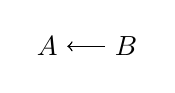
\begin{tikzpicture}
		\node (A) at (0,0) {$A$};
    		\node (B) at (1,0) {$B$};
    		\path[<-] (A) edge (B);
    		\path[->] (B) edge (A);
	\end{tikzpicture}
  }%
  \subcaptionbox{Non valid DAG}[.22\linewidth]{%
	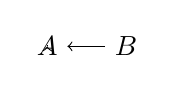
\begin{tikzpicture}
		\node (A) at (0,0) {$A$};
    		\node (B) at (1,0) {$B$};
    		\path[<-] (A) edge (A);
    		\path[->] (B) edge (A);
	\end{tikzpicture}
  }
  \subcaptionbox{Valid DAG}[.22\linewidth]{%
	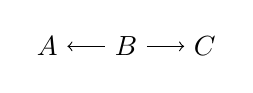
\begin{tikzpicture}
		\node (A) at (0,0) {$A$};
    		\node (B) at (1,0) {$B$};
    		\node (C) at (2,0) {$C$};
    		\path[<-] (A) edge (B);
    		\path[->] (B) edge (C);
	\end{tikzpicture}
	\label{validDAG}
  }%

\end{figure}
Bisogna inoltre capire che i DAG, essendo un metodo grafico che è per natura più sintetico, contengono molte informazioni non solo grazie agli archi disegnati ma grazie a quelli \textbf{non} disegnati, ad esempio il DAG \ref{validDAG} implica che $A \perp\!\!\!\perp C$ visto che non esiste un arco che li colleghi. %Bisogna essere molto vigili delle assunzione nascoste di un DAG.

\section{Tipi di collegamento}
Analiziamo un singolo \textit{node} in questo caso B, vediamo che se deve essere collegato ad A e C gli unici modi in cui si può collegare sono i seguenti: 
\begin{figure}[H]
\centering    
	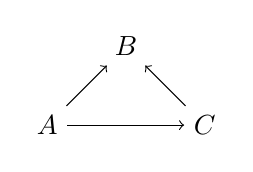
\begin{tikzpicture}
		\node (A) at (0,0) {$A$};
    		\node (B) at (1,1) {$B$};
    		\node (C) at (2,0) {$C$};
		\path[->] (A) edge (B);
    		\path[<-] (B) edge (C);
    		\path[->] (A) edge (C);
	\end{tikzpicture}
\caption{DAG: Common effect}
\label{DAG:Common effect}
\end{figure} 
\begin{figure}[H]
	\centering
	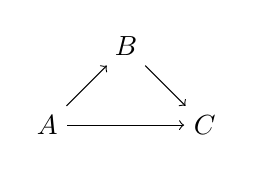
\begin{tikzpicture}
		\node (A) at (0,0) {$A$};
    		\node (B) at (1,1) {$B$};
    		\node (C) at (2,0) {$C$};
    		\path[->] (A) edge (B);
    		\path[->] (B) edge (C);
		\path[->] (A) edge (C);
	\end{tikzpicture}
\caption{DAG: Mediator}
\label{DAG:Mediator}
\end{figure} 
\begin{figure}[H]
	\centering
	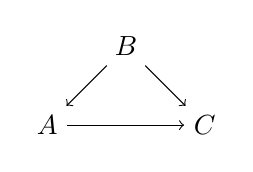
\begin{tikzpicture}
		\node (A) at (0,0) {$A$};
    		\node (B) at (1,1) {$B$};
    		\node (C) at (2,0) {$C$};
    		\path[<-] (A) edge (B);
    		\path[->] (B) edge (C);
    		\path[->] (A) edge (C);
	\end{tikzpicture}
\caption{DAG: Common cause}
\label{DAG:Common cause}
\end{figure}

Dunque B nel grafico \ref{DAG:Common effect} viene chiamato \textit{collider}, mentre B nei grafici \ref{DAG:Mediator} e \ref{DAG:Common cause} viene definito \textit{non colliders}.
Infatti se volessimo quantificare la relazione causale tra A e C quando B è un \textit{non collider} risulta più difficoltoso perchè sappiamo che B introduce correlazioni spurie tra A e C. Invece nel caso mostrato in figura \ref{DAG:Common effect} potremmo stimare esattamente come fatto nel equazione 


% magari metterli di fianco
%\begin{figure}[ht]
%  \subcaptionbox{First subfigure}[.22\linewidth]{%
%	\begin{tikzpicture}
%		\node (A) at (0,0) {$A$};
%    		\node (B) at (1,0) {$B$};
%    		\node (C) at (2,0) {$C$};
%    		\path[<-] (A) edge (B);
%    		\path[->] (B) edge (C);
%	\end{tikzpicture}
%  }%
%  \hfill
%  \subcaptionbox{Second subfigure}[.22\linewidth]{%
%	\begin{tikzpicture}
%		\node (A) at (0,0) {$A$};
%    		\node (B) at (1,0) {$B$};
%    		\node (C) at (2,0) {$C$};
%    		\path[<-] (A) edge (B);
%    		\path[->] (B) edge (C);
%	\end{tikzpicture}
%  }
%  \subcaptionbox{First subfigure}[.22\linewidth]{%
%	\begin{tikzpicture}
%		\node (A) at (0,0) {$A$};
%    		\node (B) at (1,0) {$B$};
%    		\node (C) at (2,0) {$C$};
%    		\path[<-] (A) edge (B);
%    		\path[->] (B) edge (C);
%	\end{tikzpicture}
%  }%
%
%\end{figure}

\section{Back door criterion}

\section{Collider Bias}
\begin{figure}[H]
\centering
	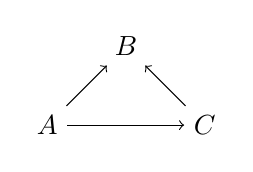
\begin{tikzpicture}
		\node (A) at (0,0) {$A$};
    		\node (B) at (1,1) {$B$};
    		\node (C) at (2,0) {$C$};
		\path[->] (A) edge (B);
    		\path[<-] (B) edge (C);
    		\path[->] (A) edge (C);
	\end{tikzpicture}
\caption{DAG:collider bias}
\label{DAG:Colliderbias}
\end{figure} 

